\documentclass[10pt,twocolumn,letterpaper]{article}

\usepackage{cvpr}
\usepackage{times}
\usepackage{epsfig}
\usepackage{graphicx}
\usepackage{amsmath}
\usepackage{amssymb}

\usepackage{graphicx}
\usepackage{caption}
\usepackage{subfigure}
\usepackage{subcaption}
\captionsetup{compatibility=false}
\usepackage{amssymb}
\usepackage{amsthm}
%\usepackage{ruler}
\usepackage{color}
\usepackage{booktabs}
%\usepackage[width=122mm,left=12mm,paperwidth=146mm,height=193mm,top=12mm,paperheight=217mm]{geometry}
\newtheorem{proposition}{Proposition}
\newtheorem{lemma}{Lemma}
%\newtheorem{proof}{Proof}
\newcommand{\RR}{\mathbb R}
\newcommand{\NNN}{\mathcal N}
\newcommand{\sumi}{\displaystyle{\sum_{i=1}^n}}
\DeclareMathOperator*{\argmin}{argmin}

% Highlighting
\usepackage{soul}
%\usepackage[usenames,dvipsnames]{xcolor}
\newcommand{\hlc}[2][yellow]{{\sethlcolor{#1}\hl{#2}}}
\newcommand{\RAF}[1]{\hlc[yellow]{(RR:) #1}}
\newcommand{\JZ}[1]{\hlc[pink]{(JZ:) #1}}
\newcommand{\PP}[1]{\hlc[green]{PP: #1}}
\newcommand{\un}[1]{\underline{#1}}

\usepackage{tikz}
\usepackage{pgfplots,pgfplotstable}
\usetikzlibrary{pgfplots.groupplots}
\pgfplotsset{grid=major,height=2in, width=\columnwidth}
\tikzset{PolySLEM/.style={mark=*, green}}
\tikzset{GaussSLEM/.style={mark=*, blue}}
\tikzset{ESVM/.style={mark=*, red}}
\tikzset{LinSLEM/.style={mark=*, black}}
\tikzset{VLAD/.style={mark=*, cyan}}
%\tikzset{ussvmne/.style={mark=None, blue, dash pattern=on 4pt off 1pt on 1pt off 1pt}}
%\tikzset{l1svm/.style={mark=*, red, mark options={solid, fill=red!80!black}, solid}}
%\tikzset{l2svm/.style={mark=*, brown!60!black, mark options={solid, fill=brown!80!black}, solid}}


% Include other packages here, before hyperref.

% If you comment hyperref and then uncomment it, you should delete
% egpaper.aux before re-running latex.  (Or just hit 'q' on the first latex
% run, let it finish, and you should be clear).
\usepackage[pagebackref=true,breaklinks=true,letterpaper=true,colorlinks,bookmarks=false]{hyperref}

% \cvprfinalcopy % *** Uncomment this line for the final submission

\def\cvprPaperID{882} % *** Enter the CVPR Paper ID here
\def\httilde{\mbox{\tt\raisebox{-.5ex}{\symbol{126}}}}

% Pages are numbered in submission mode, and unnumbered in camera-ready
\ifcvprfinal\pagestyle{empty}\fi
\begin{document}

%%%%%%%%% TITLE
\title{Kernel Square-Loss Exemplar Machines}

\author{Rafael S. de Rezende\\
INRIA Paris\\
Institution1 address\\
{\tt\small rafael.sampaio_de_rezende@inria.fr}
% For a paper whose authors are all at the same institution,
% omit the following lines up until the closing ``}''.
% Additional authors and addresses can be added with ``\and'',
% just like the second author.
% To save space, use either the email address or home page, not both
\and
Second Author\\
Institution2\\
First line of institution2 address\\
{\tt\small secondauthor@i2.org}
}

\maketitle
%\thispagestyle{empty}
%%%%%%%%% ABSTRACT
\begin{abstract}
This paper proposes an extension of the exemplar SVM (ESVM) as a novel approach to feature encoding for feature retrieval applications.
%This paper proposes a new feature encoding pipeline, based on the success of the exemplar SVM (ESVM) \cite{ZePe15} and linear discriminant analysis (LDA) as whitening \cite{HMR12}.
We first show that, by replacing the hinge-loss by the square-loss in the ESVM cost function, equivalent results in image retrieval can be obtained at a fraction of the computational cost. 
We call this model square-loss exemplar machine, or SLEM. 
We also introduce a kernelized SLEM which can be implemented efficiently through a low-rank matrix decomposition and
%benefits from the same computational advantages but 
displays improved performance. 
Both SLEM variants exploit the fact that the negative examples are fixed for all the positives in the training set, so most of the SLEM computational complexity is relegated to an offline process independent of the positive examples. 
Our experiments establish the performance and computational advantages of our approach using a large array of base feature representations and standard image retrieval datasets.
\end{abstract}

\section{Introduction}



An effective image 
representation is a crucial component of image retrieval systems
where, given some query image,  images must be retrieved from a large 
database, then ranked according to their degree of similarity with the 
query.
%Robust image representations are a crucial component of a vast number of computer vision applications. 
%Within these, the \emph{image retrieval} application is an important example wherein a query image is provided to the system, which must in turn find all matching images from within a large, unannotated database. 
The matching process is done entirely based on the pixel content of the query and database images, and the search must be robust to large image variations due to camera pose, color differences and scene illumination, amongst others.


The advances in image representation enabled the success of new systems in this challenging task. %An image representation function commonly maps a given input image to a vector in a fixed dimensional space called the image \emph{feature vector}. 
Indeed, many successful feature representations for image retrieval rely on unsupervised models such as $K$-means \cite{Delhumeau2013} or Gaussian mixture models \cite{Perronnin2010} and, before the neural networks \textit{renaissance}, these representations would outperform methods that exploit supervised learning of image features directly~\cite{Bilen2015,Rana}.
Today, with the popularization of convolutional architectures, global image descriptors are often obtained by aggregation and/or pooling the last convolutional layers \cite{babenko15,GoAlReLa16,KaMeOs16} or by addition of new differentiable layers to an existing architecture~\cite{Arandjelovic15}.
%One of the main reasons for this is the lack of adequately large and varied supervised datasets that are expensive to collect.
%A now pervasive example of an image feature representation is that consisting of the activation coefficients extracted from the previous-to-last layer of Convolutional Neural Networks (CNNs) \cite{Krizhevsky2012}. Although CNNs are trained in a fully-supervised manner for the image classification task, they have been shown to transfer well not only to new, unseen classes \cite{Oquaba,Chatfield2014}, but also to alternate tasks such as object detection \cite{Girshick2014} and, importantly, image retrieval \cite{Sharif}.

The exemplar support vector machine (ESVM), originally proposed by Malisiewicz {\it et al.} \cite{Malisiewicza}, leverages the availability of large, unannotated pools of images within the context of supervised learning. It uses a large generic pool of images as a set of negative examples, while using a single image (the \emph{exemplar}) as a positive example. Given these training sets, an SVM classifier is learned that can  generalize well, despite the drastically limited size of the set of positive examples.

Zepeda \emph{et al.} \cite{ZePe15} propose to treat instead the weights of the resulting classifier as a new feature vector for image retrieval. %This new ESVM feature is derived from \emph{base} feature representations ({\it e.g.,} CNN activation features) of the exemplar and the negative pool.
%An extension \cite{ZePe15} of the ESVM formulation discussed above instead treats the resulting  classifier as an \emph{enhanced} representation of the image feature representing the exemplar image (the \emph{base} feature representation).
An ESVM feature is extracted from each database image, as well as from the query image, by treating each image as an exemplar while keeping a fixed pool of generic negative images. Searching amounts to computing distances between the query and the database ESVM features. Note that ESVM features can be derived from arbitrary \emph{base} features ({\it e.g.}, CNN activations) of the exemplar and the images in the generic negative pool. %An interesting interpretation of this approach is that the ESVM features represent what is unique about the exemplar relative to the pool of generic negatives, which is the role of a classifier.


One important drawback of the ESVM feature encoding approach is that computing the  classifier requires solving an optimization problem for each positive example (\ie each query and each database image). This can be time consuming for the large negative pool sizes required for good ESVM feature performance. In this work we propose using the square loss instead of the hinge loss, in effect converting the ESVM problem into a ridge regression that can be solved in closed form. The parameters of the corresponding classifier, which we call the square loss exemplar machine (SLEM), had been shown to both generalize LDA \cite{Koba15} and, for the general case of multiple positive samples (LS-SVM)~\cite{lssvm}, form features with comparable binary classification performance while drastically reducing the computational cost.


Since computing the SLEM features requires inverting a large matrix related to the training set's covariance matrix, we propose an efficient way to compute this inverse that exploits the fact that only a single (positive) example changes in the training set when computing SLEM features for different images. We show experimentally that our representation matches and even improves upon the performance of ESVM features on two standard datasets using a wide range of base features.

We also introduce a kernelized variant of SLEM that enjoys similar computational advantages but improves retrieval performances. Further computational efficiency is obtained using a kernel principal components analysis (KPCA) decomposition of the negative samples.
%low rank incomplete Cholesky decomposition of the negative pool kernel matrix.

The rest of this paper is organized as follows:
%In Section \ref{prior work} we provide an overview of various existing feature representation methods. 
In Section \ref{lsesvm} we first review the original ESVM feature representation method and subsequently introduce the proposed linear SLEM model. We then introduce the kernelized SLEM variant in Section \ref{nonlinear SLEM}. We then present the low-rank approximation of our method that enables efficient implementations in the non-linear case in Section \ref{eff_imp}. We evaluate our proposed method in image retrieval in Section \ref{eval}, and present conclusions in Section \ref{conclusion}.



% Image search
% - Importance.
% - Feature representations. 

% Feature representation - supervised learning
% - Generic framework.
% - Deep CNN features.
% - ImageNet.

% Image retrieval
% - Supervised - Eusipco, NetVLAD.
% - VLAD, Fisher.
% - Cheaper.

% Pool:
% LDA
% SVMs for feature representations - parts learning, Malizsiewics


%\section {Introduction}
% The exemplar SVM (E-SVM) was first introduced by Malisiewicz et al. in \cite{Efros11} as a conceptually simple framework for object detection and image classification where the training set has a small ratio of positive/negative examples. 
% At training time, many SVMs are learned from a large pool of negative against a single positive (so called exemplar). 
% At test time, the scores of the test images for each classifier are fitted by a logistic regression. 
% The final score of an image is then a non-linear combination of scores from multiples exemplar SVMs.

% They have also been used in \cite{Efros12} in image retrieval tasks, using the classifier score to rank matching candidates.
% However this transfer of information from classification to retrieval is severely limited. 
% Indeed, the purpose of a support vector machine is to separate positive and negative samples, i.e., predict discrete labels. 
% The distance between a negative sample and the classification hyperplane has no value as a measure of has \emph{a priori} no value of continuous matching score.

% Zepeda et al. address this problem in \cite{ZePe15} by firstly, performing an E-SVM to each image in a dataset instead of only for the query images and secondly, comparing its classifiers distance to the query's classifier instead of comparing scores. 
% These modifications guarantee we are ranking distances between two points instead of classification scores.
% Therefore \cite{ZePe15} refers to E-SVMs as features encoders: a pipeline that takes an image representation as input and returns an improved image representation. This type of feature enhancing is more akin to methods such as whitening, PCA and LDA.

% This paper introduces the square-loss Exemplar machine (SLEM), which consists of optimizing the same cost function of a regular E-SVM where the hinge loss is replaced by the square loss. 
% The square loss version has the advantage of having a much more efficient optimization. Indeed, the minimization of its cost function is solved by a linear system and can be done for all exemplar simultaneously, whereas the regular E-SVM cost function is generally minimized one exemplar at a time, normally by stochastic gradient descent \cite{bottou10}.
% Also, for the machine learning tasks of binary classification, both regular SVM and least-squares SVM have similar performances \cite{YeXi07}.
% %Also, for the machine learning tasks of binary classification, both regular SVM and least-squares SVM have the same performance if positive and negative samples are separable and the pool of samples is linearly independent \cite{YeXi07}. 
% We also introduce a kernelized version of SLEM, efficiently implemented, that gives better results and superior scalability for large-scale image retrieval problems.

%%% Local Variables:
%%% TeX-master: "main_eccv"
%%% End:


%\section{Prior work}
\label{prior work}

\begin{verbatim}
Classic features:
-----------------
VLAD
Fisher Vector
Triangulation embedding
Tolias

Enhancements:
-------------
Spatial Pyramid Pooling (SPP)
Hellinger kernel / root SIFT
Dense sampling
E-SVM

New features:
-------------
CNN features
NetVLAD

Hybrid pooling CNN / aggregator features:
-----------------------------------------
VLAD orderless pooling (exploits SPP)
Conv layers + aggregator: Vedaldi, Kulkarni
SIFT + FCs: Perronin
unsup dense: Deep Fisher vector.


Kernel methods
--------------
\end{verbatim}

% \emph{\color{red} paragraph about image search}

% The image retrieval litterature 

% %where the query image is the positive example and the rank of an search result image is the score of the score of this image in the classifier obtained by the E-SVM. 

% The application of kernel methods for SVM has an extensive bibliography. \emph{\color{red} so extensive that I do not know yet what to put here...}

%%% Local Variables:
%%% TeX-master: "main_eccv"
%%% End:

\section{Square loss exemplar machine}\label{lsesvm}
In this section, we revisit the exemplar SVM model presented by \cite{Efros11} as an instance of a more general family of classifiers. Then, we introduce the square loss exemplar machine (SLEM) by solving a simple variant this model and study its properties.
\subsection{Exemplar classifiers} \label{esvm}
We are given base features in $\RR^d$ at training time, one positive example $x_0$ in $\RR^d$ and a set of negative examples $X = [x_1, x_2,...,x_n]$ in $\RR^{d\times n}$, each column of $X$ representing one example by a vector in $\RR^d$. 
We are also given a loss function $l:\{-1, 1\}\times \RR\rightarrow\RR^+$. Learning an exemplar classifier from these examples amounts to minimizing the function 
\begin{equation}
J(\omega, \nu) = \theta \ l(1, \omega^Tx_0+\nu) +\dfrac{1}{n}\sumi l(-1, \omega^T x_i+\nu)+\dfrac{\lambda}{2}\|\omega\|^2, 
\label{eq:first}
\end{equation}
w.r.t. $\omega$ in $\RR^d$ and $\nu$ in $\RR$. In Eq. (\ref{eq:first}), $\lambda$ and $\theta$ are respectively a regularization parameter on $\omega$ and a positive scalar adjusting the weight of the positive exemplar.
%\footnote{We could also acknowledge a parameter $\theta$ other than $\frac{1}{n}$ as a regularization to the error of each negative example. But this parameters seems to be less important to cross-validate. Also, setting $\theta=\frac{1}{n}$ simplify Equation (\ref{omega:solution}) and allows the use of Woodbury identity.} 

Given a cost $l$, we define the correspondent \emph{exemplar classifiers} of $x_0$ with respect to $X$ are the weights $\omega^\star(x_0,X)$ that minimizes the loss function $J$:
\begin{equation}
\big(\omega^\star, \nu^\star\big) = \underset{(\omega,\nu)\in\RR^d\times\RR}{\argmin} \ J(\omega, \nu). \footnote{Depending on the loss function $l$, $\nu^\star(x_0,X)$ may be not unique.}
%\big(\omega^\star(x_0, X), \nu^\star(x_0, X)\big) = \underset{(\omega,\nu)\in\RR^d\times\RR}{\argmin} \ J(\omega, \nu). 
\label{omega:first}
\end{equation}
%To shorten the notation, we refer to these solutions as $\omega^\star$ and $\nu^\star$ when their arguments are implicit.

%\cite{Efros11} introduced ensembles of exemplar classifiers for object detection, but single exemplar classifiers have been used as replacement of the original feature $x_0$ for image classification and retrieval \cite{ZePe15} and detection \cite{GMPD12}. \RAF{Maybe this should be in the introduction instead.}
The exemplar SVM~\cite{Efros11,Efros12} is an instance of this model where $l$ is the hinge-loss. 
%Applications of ESVM use the hinge loss function, which guarantees that $J$ is a convex function. 
The solution of Eq. (\ref{omega:first}) can be thus found by stochastic gradient descent~\cite{bottou10} individually for each positive sample. The next subsection show how to calculate all exemplar classifiers simultaneously by changing the loss function.

\subsection{Square loss function}\label{slem:intro}
Now, let us study the same learning problem for the square-loss function $l(y,\hat{y}) = \frac{1}{2}(y-\hat{y})^2$. As in the case of the hinge loss, Equation (\ref{eq:first}) is a convex problem. 
However it is now a ridge regression problem, whose unique solution can be found in closed form as
\begin{align}
\begin{cases}
\vspace{3 mm}
\omega^\star &= \dfrac{2\theta}{\theta+1}U^{-1}(x_0-\mu), \\
%\vspace{3 mm}
\nu^\star &= \dfrac{\theta-1}{\theta+1}-\dfrac{1}{\theta+1}(\theta x_0+\mu)^T\omega^\star,
\end{cases}
\label{omega:solution}
\end{align}
%\begin{align}
%\nu^\star &= \dfrac{\theta-1}{\theta+1}-\dfrac{1}{\theta+1}(\theta x_0+\mu)^T\omega^\star, \label{eq:nustar}\\
%\omega^\star &= \dfrac{2\theta}{\theta+1}U^{-1}(x_0-\mu) \label{eq:wstar}
%\end{align}
where:
\begin{align}
\begin{cases}
\mu = &\frac{1}{n}\sum_{i=1}^n x_i,\\ \\
U = &\frac{1}{n}XX^T-\mu\mu^T\\
&+\frac{\theta}{\theta+1}(x_0-\mu)(x_0-\mu)^T+\lambda\mathrm{Id}_d. \label{eq:U}
\end{cases}
\end{align}
Equation (\ref{omega:solution}) shows how to solve (\ref{eq:first}) simultaneously for all exemplars.
\cite{lssvm}
%Replacing the hinge loss by the square loss offers a more compact solution, but not necessarily more efficient.

\textbf{Woodbury identity.} 
We can simplify Eq. (\ref{omega:solution}) by modifying $U$ in Eq. (\ref{eq:U}).
Let us define $A = \frac{1}{n}XX^T-\mu\mu^T +\lambda\mathrm{Id}_d$ our regularized covariance matrix and assume its inverse $A^{-1}$ known. 
%$A$ is the covariance matrix of the negative samples $X$\footnote{added of a small term proportional to the identity matrix to insure $A$ is positive-definite.}. Let us assume its inverse $A^{-1}$ is known. 
The matrix $U$ now reads $U = A + \frac{\theta}{\theta+1}\delta\delta^T$, where $\delta=x_0-\mu$ is the centralized (w.r.t. the negatives' mean) positive sample. The Woodbury identity \cite{woodbury} gives us
\begin{equation}
U^{-1} = A^{-1} -\dfrac{\theta}{\theta\delta^TA^{-1}\delta+ \theta+1}A^{-1}\delta^T\delta A^{-1}. \label{invU}
\end{equation}
Substituting (\ref{invU}) in (\ref{omega:solution}) yields
\begin{equation}
\begin{split}
\omega^\star &= \dfrac{2\theta}{\theta +1}\left(A^{-1}\delta - \dfrac{\theta}{\theta\delta^TA^{-1}\delta+ \theta+1} A^{-1}\delta (\delta^TA^{-1}\delta)\right)\\
&= \dfrac{2\theta}{\theta\delta^TA^{-1}\delta+ \theta+1} A^{-1}\delta.\label{Wood:omega}
\end{split}
\end{equation}

Note that the positive sample weight $\theta$ does not influence the direction of the optimal vector $\omega^\star$, only its norm. This means that if search and ranking are based on the normalized feature $\frac{1}{\|\omega^\star\|}\omega^\star$, $\theta$ does not influence the matching score of the SLEM vectors of two different images. This sets SLEM appart from ESVM which requires this parameter to be calibrated \cite{Efros11,ZePe15}. We can thus set $\theta=\frac{1}{n}$ for the remaining of this work.
%The normalized exemplar classifier $\omega^\star$ is therefore a linear transformation of $x_0-\mu$.
%Indeed, if $\omega$ and $\omega'$ are the $d$-dimensional SLEM vectors of $x$ and $x'$, respectively, their cosine similarity reads:
%we can denote $s$ the matching score scalar function defined in $\RR^d\times \RR^d$, which is given by
%\begin{equation}
%s(\omega, \omega') = \dfrac{\omega^T \omega'}{\|\omega\| \|\omega'\|} = \frac{(x-\mu)^TA^{-2}(x'-\mu)}{\|A^{-1}(x-\mu)\|\|A^{-1}(x'-\mu)\|},\label{match:score}
%\end{equation}
%which does not depend on the value of $\theta$. 
%This means that the weight of the positive sample can be fixed at any positive value without changing matching scores. 

\subsection{LDA and SLEM}\label{sec:lda}

It is interesting to note the relationship between SLEM and the classical linear discriminant analisys (LDA).
Let us reanalyse Eq. (\ref{eq:first})) an suppose that we have multiple positive samples. It can be shown that in this case, the corresponding linear classifier of Eq. (\ref{eq:first}) for the square-loss is also given by
(\ref{omega:solution}), where $x_0$ denotes this time the center of mass
of the positive samples {\em if} these samples have the {\em same} covariance matrix $\Sigma$ as the negative samples $X$.
 
This equal-covariance assumption is of course quite restrictive, and probably unrealistic in general. It is interesting to note, however, that this is exactly the assumption made by linear discriminant analysis. As shown in~\cite{Hastie2009} for example, LDA can be seen as a (non-regularized) linear classifier with decision function $\omega^T_{LDA} z+ \nu_{LDA}$, where $z$ is a sample in
$\RR^d$, and
\begin{equation}
\left\{\begin{array}{l}
\displaystyle \omega_{LDA}=\Sigma^{-1}(x_0-\mu),\\
\displaystyle \nu_{LDA}=-\frac{1}{2}(x_0+\mu)^T \omega_{LDA},
\end{array}\right.
\label{eq:lda}
\end{equation}
 
This shows that SLEM is a generalized version of LDA: Indeed, when $\lambda=0$ in SLEM (i.e. no regularization), $A = \Sigma$, the vectors $\omega_{LDA}$ of Eq. (\ref{eq:lda}) and $\omega^\star$ of Eq. (\ref{Wood:omega}) have the same direction.
%This observation has been equally made by \cite{Koba15}.
Many interesting properties of LDA has been used recently for classification tasks \cite{GMPD12,HMR12} and, more recently, for image retrieval with convolutional neural network activations \cite{babenko15}.
With our simple generalization of LDA, we hope to obtain superior results.

%In the next section, we take one step further and generalize SLEM with kernel methods. \hlc{something to add to this sentence?}


%%% Local Variables:
%%% TeX-master: "main_eccv"
%%% End:


\section{The kernel SLEM}
\label{nonlinear SLEM}

\subsection{Kernel methods}\label{kernel:review}
Let us recall a few basic facts about kernel methods for supervised
classification. We consider a reproducing kernel Hilbert space (RKHS)
$H$ formed by real functions over some set
$X$, and denote by $k$ and $\varphi$ the corresponding reproducing kernel and feature map (which may not admit a known explicit form) over $X$, respectively. We
address the following learning problem over $H\times\RR$:
%\begin{equation}
%\min_{h\in H,\nu\in\RR}
%\sum_{i=1}^n l(y_i,h(x_i)+\nu) + \frac{\lambda}{2}\|h\|_H^2,
%\label{eq:kernel}
%\end{equation}  
%By definition of a reproducing kernel,
%Equation (\ref{eq:kernel}) can be rewritten as
\begin{equation}
\min_{h\in H,\nu\in\RR}
\dfrac{1}{n}\sum_{i=1}^n l(y_i,\langle \varphi(x_i),h\rangle+\nu) +
\dfrac{\lambda}{2}\|h\|_H^2,
\label{ker:aff}
\end{equation} 
where the pairs $(x_i,y_i)$ in $X\times \{-1,1\}$, $i=1\dots n$ are training samples, %and $l: \{-1,1\}\times \RR\rightarrow\RR^+$ is some arbitrary loss function. 
%$\varphi$ is the {\em feature map} over $X$ associated with the kernel $k$ (which may not admit a known explicit form) 
and $\langle h, h' \rangle$ is the inner product of element $h$ and $h'$ in $H$. We dub problems with the general form of (\ref{ker:aff}) {\em affine}
supervised learning problems since, given some fixed element $h$ of
$H$ and some scalar $\nu$, $\langle h,h'\rangle+\nu$ is an affine function of $h'$,
whose zero set defines an affine hyperplane of $H$ considered itself
as an affine space.

Let $K$ denote the kernel matrix with entries $k_{ij}=\langle\varphi(x_i),
\varphi(x_j)\rangle$ and rows $k_i^T=[k_{i1}, k_{i2},...,k_{in}]$, $i$ in $\{1,\ldots,n\}$.  We assume from now on that $l$ is convex and continuous. Under this assumption, Eq. (\ref{ker:aff}) admits an equivalent formulation
\begin{align}
\min_{\alpha\in\RR^{n}, \ \nu\in\RR} \left(\dfrac{1}{n}\sumi l(y_i, k_i^T\alpha+\nu)  +\dfrac{\lambda}{2}\alpha^TK\alpha\right), \label{ker:first}
\end{align}
and any solution $(\alpha^\star,\nu^\star)$ to (\ref{ker:first})
provides
a solution $(h^\star,\nu^\star)$ to (\ref{ker:aff}) with
$h^\star=\sum_{i=1}^n \alpha_i^\star\varphi(x_i)+\nu^\star$. This result follows from the Riesz representation theorem~\cite{SHS01,Wahba90}.


%where $K$ is a $(n+1)\times (n+1)$  matrix and $k_i$ is its $(i+1)$-th column matrix for $i$ in $\{0, 1, ..., n\}$.\\



Assuming our reproducing kernel is semidefinite positive, 
%\footnote{\textit{i.e.} for any $z$ in $\RR^n$, $z^TKz\ge 0$. This is equivalent to all eigenvalues of $K$ being non-negative.} 
$K$ is a semidefinite positive matrix and can be decomposed as $K=BB^T$.
%, with $B$ a rank $r$ upper triangular matrix of size $n\times r$. 
Using this factorization, the kernelized problem can be expressed as 
\begin{equation}
\min_{\beta\in\RR^r,\nu\in\RR} \left( \dfrac{1}{n}\sumi l(y_i, b_i^T\beta+\nu)+\dfrac{\lambda}{2}\|\beta\|^2\right), \label{beta:first}
\end{equation}
where $b_i^T$ denotes the $i$-th row of $B$ and $r$ is the number of columns of $B$. 
If $(\beta^\star, \nu^\star)$ is the solution Equation (\ref{beta:first}), the corresponding vector $\alpha^\star$ (or, more correctly, \textit{a} corresponding vector of dimension $n\geq r$) 
can be computed by $\alpha^\star=P\beta^\star$, where $P$ is the pseudoinverse of $B^T$.

Note that Eq. (\ref{beta:first}) allows us to write the kernel learning problem (\ref{ker:aff}) as an instance of Eq. (\ref{eq:first}) by setting $y_i=-1$ for all but one training sample. For our approach, we wish to solve (\ref{beta:first}) for many positive training samples (one at a time) against the same set of negative training samples. In the following subsections, we show how to take advantage of the fixed negative samples to efficiently solve (\ref{beta:first}).

\subsection{Offline preprocess of negative samples}\label{offline}
In order to calculate offline all operations that are dependent only on negative samples, let us suppose that the positive training sample is unknown and $K$ is the kernel matrix of the negative samples $X$.
The preprocessing phase consists of the calculation of the decomposition $B$ and the constants of Eq. (\ref{Wood:omega}): $\mu = \frac{1}{n}\sum_{i=1}^n b_i^T$ and $A = \frac{1}{n}B^TB-\mu\mu^T +\lambda\mathrm{Id}_r.$
These operations are done offline and their results are stored. In the processing of positive samples, \emph{i.e.} the online phase, these results are loaded.
%Equation (\ref{beta:first}) has the same structure of Eq. (\ref{eq:first}) if we were to consider $\theta=0$ and all labels $y_i=-1$.

\subsection{Online addition of a positive sample}
\label{subsec:adding}
We now wish to write Eq. (\ref{beta:first}) as an exemplar classifier, with one positive example $x_0$ and $n$ negative examples $X$.
%Let us assume the factor $B$ is given. %The calculation of a kernel Cholesky factorization is solved efficiently by \cite{BaJo05,BaJo02}. 
%We further analyse how to compute this factorization in subsection \ref{offline}.
We denote by $K'$ the augmented kernel matrix obtained by adding the positive samples $x_0$. Such a matrix can be written as
\begin{equation}
K' = \begin{bmatrix}
k_{00} & k_0^T\\
k_0 & K
\end{bmatrix},
\end{equation}
where $k_{00}=\langle \varphi(x_0),\varphi(x_0)\rangle$ is a scalar and $k_0= [\langle \varphi(x_0),\varphi(x_i)\rangle]_{1\le i\le n}$ is a vector in $\RR^n$. 
The following lemma show how the factorization of $K'$ can be derived from the factorization of its sub-matrix $K$ and the solution of a $n\times n$ linear system.

\begin{lemma} The augmented kernel matrix $K'$ can be factorized as $K'= B'B'^T$ with
%\begin{align}
%K'&= B'B'^T,\quad\text{where}\quad
%B'=\begin{bmatrix}
%u & v^T\\0 & B
%\end{bmatrix}\\
%v&=B^\dagger k_0,\,\, u=\sqrt{k_{00}-||v||^2}.\label{eq:lemma1}
%\end{align}
\begin{equation}
B'=\begin{bmatrix}
u & v^T\\0 & B
\end{bmatrix},~
v = B^\dagger k_0,~ u=\sqrt{k_{00}-||v||^2}.
\label{eq:lemma1}
\end{equation}
\end{lemma}\label{lemma1}
\begin{proof}
For $B'$ defined by (\ref{eq:lemma1}), we have that
\begin{equation}
B'B'^T = 
\begin{bmatrix} u^2+\|v\|^2 & v^TB^T\\ 
Bv& BB^T\end{bmatrix} 
=\begin{bmatrix} k_{00} & v^TB^T\\ 
Bv& K\end{bmatrix} .
\end{equation}
Since $K'$ is positive semidefinite, $k_0$ must lie in the column space $\mathcal{B}$ of $B$.
%\footnote{
Indeed, if we suppose $k_0$ does not belong to $\mathcal{B}$, then it can be decomposed uniquely as $k_0=s+t$, $s\in\mathcal{B}$ and  $t\in\mathcal{B}^\perp$, with $t\ne 0$. In one hand, $K'$ being semidefinite positive implies that $[1, -at^T]K'[1; -at]=k_{00}-2a\|t\|^2\ge 0$ for all real value $a$. In the other hand, for $a$ large enough, $k_{00}-a\|t\|^2\le 0$, which is a contradiction.
%} 
Hence $v=B^\dagger k_0$ is an exact solution of $Bv=k_0$. The fact that $k_{00}-\|v\|^2$ is non-negative comes from the fact that the Schur complement $K-k_0 k_0^T / k_{00}$ of $k_{00}$ in $K'$ is itself positive semidefinite.
%\footnote{
Indeed, since the matrix $k_{00}K-k_0k_0^T=B(k_{00}\mathrm{Id}_r-vv^T$ is also positive semidefinite. Thus $v^T(k_{00}\mathrm{Id}_r-vv^T)v = \|v\|^2(k_{00}-\|v\|^2)\ge 0$. \qedhere
%}
\end{proof}


This lemma allows us to add a positive sample to Eq. (\ref{beta:first}).
%$\beta^\star(x_0,X), \nu^\star(x_0,X) = \underset{\beta\in\RR^{r+1}, \nu\in\RR}{argmin}J'(\beta, \nu)$, for
With a positive exemplar, Eq. (\ref{beta:first}) now reads
\begin{align}
 \dfrac{1}{n}l(1, b_0'^T\beta+\nu) +\dfrac{1}{n}\sumi l(-1,b_i'^T\beta+\nu)
+\dfrac{\lambda}{2}\|\beta\|^2,\label{beta:final}
\end{align}
with $b_i'^T$ being the $(i+1)$-th row of $B'$, $i$ in $\{0,1,...,n\}$. In particular, $b_0'=[u; \ v]$ and, for $i>0$, $b_i'=[0; \ b_i]$. The solution $(\beta^\star,\nu^\star)$ in $\RR^{r+1}\times\RR$ can be computed just as before by Equation (\ref{omega:solution}), replacing $x_0$ by $b_0'$, $\mu$ by $\mu' = \frac{1}{n}\sum_{i=1}^n b_i'$ and $X$ by the $(r+1)\times n$ matrix $Q$ of columns $b_1', b_2',...,b_n'$. $\alpha^\star$ is now calculated as
$\alpha^\star=P'\beta^\star$, where $P' = [u^{-1} \ 0^T; -u^{-1}Pv \ P]$ is the pseudoinverse of $B'^T$. 
%This can be expressed by the linear system


\subsection{Similarity score}\label{simi_score}
Once the optimal parameters $(\beta, \nu)$ from (\ref{beta:final}) and the coordinates $u$, $v$ of $b_0'$ from (\ref{eq:lemma1}) have been found\footnote{We drop the ``$\star$'' in this subsection to avoid cluttering the notation.}, they can be used directly for measuring similarity between matching images.

Indeed, suppose two image descriptors $x_0$ and $x_0'$ are given and we wish to calculate the similarity score between theirs SLEM representations $h$ and $h'$, denoted by $s(h,h')$. 
We write $h'=\alpha_0'\varphi(x_0')+\sum_{i=1}^n \alpha_i'\varphi (x_i)+\nu'$. 
Moreover, $\alpha$ can be expressed by the linear system
\begin{equation}
\begin{bmatrix} \alpha_0 \\ \hat{\alpha} \end{bmatrix} = \begin{bmatrix} \frac{1}{u} & 0^T \\-\frac{1}{u}Pv & P  \end{bmatrix} \begin{bmatrix}\beta_0 \\ \hat{\beta} \end{bmatrix}.\label{alpha:to:beta}
\end{equation}
Using Eq. (\ref{alpha:to:beta}) and ignoring bias $\nu$ and $\nu'$ which have empirically no influence, $s(h,h')$ is given by:
\begin{equation}
\begin{split}
s(h,h') & = \langle h, h'\rangle \\
		& = \hat{\alpha}^{T} K\hat{\alpha}'+\alpha_0k(X, x_0)^T\hat{\alpha}'+\alpha_0'k(X, x_0')^T\hat{\alpha} \\
		& \ \ \ \ \ +\alpha_0\alpha_0'k(x_0,x_0')\\
		& = \hat{\beta}^T\hat{\beta}'+\lambda^{-2}(k(x_0,x_0')-v^T).
		%& = \hat{\beta}^T\hat{\beta}'+\frac{\beta_0\beta_0'}{uu'}(k(x_0,x_0')-v^T).
\end{split}
\end{equation}

For a given image whose descriptor is $x_0$, we need to store $x_0$, $\hat{\beta}$ and $v$ to calculate its matching score to whichever other image for SLEM. Each image depends therefore on a vector of $p+2r$ dimensions.

%%% Local Variables:
%%% TeX-master: "main_eccv"
%%% End:



\section{Efficient implementation}\label{eff_imp}

\begin{figure*}[!t]
\begin{centering}
\begin{tikzpicture}
    \begin{groupplot}
      [group style={%
        columns=2,
        rows=1,
        group name=plots,
        xlabels at=edge bottom,
        %y descriptions at=all,
        horizontal sep=4em,        
      },
      enlarge x limits={abs=.1},
      width=0.5\textwidth,
      height=0.4\textwidth,
      ]
    \nextgroupplot[xlabel=Decomposition rank.,
		ylabel=Residue,
		domain=1:1000]
        \addplot[blue] table {valB.dat};
        \addlegendentry{KPCA}
        \addplot[red] table {valR.dat};
        \addlegendentry{ICD}
        \addplot[green] table {valG.dat};
        \addlegendentry{CCD}
        
    \nextgroupplot[xlabel=Decomposition rank.,
		ylabel=Time in s,
		domain=1:1000]
        \addplot[blue] table {lineB.dat};
        \addplot[red] table {lineR.dat};
        \addplot[green, mark=*] coordinates{(999, 0.1532)};
        
    %\nextgroupplot[xlabel=Decomposition rank,
	%	ylabel=Time in s,
	%	domain=1:1000]
	%	\addplot[blue]\addplot[blue] table {valB.dat};
    %    \addplot[red] table {valR.dat};
    %    \addplot[green] table {valG.dat};
        
    \end{groupplot}    
\end{tikzpicture}
\caption{Comparison between complete Cholesky decomposition (CCD, in green), incomplete Cholesky decomposition (ICD, in red) and kernel PCA (KPCA, in blue), varying the rank of $B$. Left: Residue for each decomposition. Right: Time of calculation. We use SPoC features~\cite{babenko15} of 1000 sample images.}
\label{fig:residue}
\end{centering}
\end{figure*}

When compared to the linear square-loss classifier of Section \ref{slem:intro}, one drawback of a kernelized approach is that the dimension of our problem grows with the size $n$ of the negative samples.
The offline factorization $B$ of $K$ demands $O(nr)$ storage and at best $O(nr^2)$ time. This factorization can be obtained in different ways, depending on the aspect we wish to optimize. Efficiency in time and efficiency in storage are the two most common of these aspects. In this section we propose three different decompositions of $K$, to be applied depending on whether we want to minimize time or storage.
%on which of these two efficiencies we hope to achieve.

%As for the online step, solving Equation (\ref{beta:final}) amounts to, for all positive exemplars, calculating the row $[u, v^T]$ of $B'$  from Lemma 1 and solving a linear system in $A$, which is a $(r+1)\times (r+1)$ matrix. The first of these is computed in time $O(nr)$ and the second, $O(r^3)$.


\subsection{Time-efficient implementation}
The Cholesky decomposition is the most used factorization of positive-semidefinite matrices in kernel-based learning \cite{BaJo02,BaJo05,FiSc01}. 
The computation of the factor $B$ depends on a permutation $\pi(n) =\{i_1,i_2,\dots,i_n\}$ of $\{1,2,\dots, n\}$, called \textit{pivots}. The $t$-th column of $B$ is calculated iteratively as:

\begin{align}
\begin{cases}
\vspace{3 mm}
B(i_t, t) = \left(K(i_t,i_t)-\sum_{m=1}^{t-1} B(i_{m},m)  \right)^{\frac{1}{2}},\\
\vspace{3 mm}
B(i_j,t) = 0,\\
B(i_j, t) = \frac{1}{B(i_t,t)}(K(i_j,i_t)  -\sum_{m=1}^{t-1}B(i_j,m)B(i_t,m)), \end{cases}\label{icd:algo}
\end{align}
for all $t<j\le n$. There are two possible choices of Cholesky decomposition. The incomplete Cholesky decomposition (ICD) stops its algorithm after $r$ steps and has complexity $O(nr^2)$. 
To minimize the residue $\mathrm{tr}(K-BB^T)$, the $t$-th pivot is calculated at the end of the $t$-th interaction. 
In the other hand, the complete Cholesky decomposition (CCD) consists of a full-rank decomposition, \textit{i.e.} the rank $r$ of $B$ is equal to $n$ and it has complexity $O(n^3)$. 
In this case, the pivots are irrelevant to the final residue (which is zero) and can be assumed to be $i_t=t$. %The computation of pivots makes CCD more efficient for similar residues.
We compare CCD and ICD performances in Fig. \ref{fig:residue}. We see that for small $r$, ICD is indeed faster. As we increase the value fo $r$, ICD becomes slower than CCD due to the pivot calculation but its residue decreases. We further compare both methods in Section \ref{time-scale}.

We make sure $K$ is positive-definite by adding $\epsilon$ to its diagonal, where $\epsilon=\min(0,-\lambda_{min})$ and $\lambda_{min}$ is the smallest eigenvalue of $K$. Therefore, from the equation $BB^T=K+\epsilon\mathrm{Id}_n$, $B$ has rank $n$ and we can apply CCD.

\subsection{Storage-efficient implementation}\label{low-rank} %/Low-rank decomposition} 
Let us now consider instead the problem of improving storage efficiency. As discussed in section \ref{simi_score}, for each positive exemplar we store its original encoding plus a $2r$ vector, so we aim to decompose $K$ at a small rank $r$.
For small values of $r$, a kernel PCA (KPCA) factorization guarantees a better approximation of $K$ than the Cholesky decomposition at a higher time cost. Indeed, as illustrated in Figure \ref{fig:residue}, a kernel PCA gives smaller residues than ICD at small rank. We plot the ratio $\mathrm{tr}(K-BB^T)/\mathrm{tr}(K)$ when we vary the number of columns $r$ of $B$, and we see a faster convergence for the kernel PCA decomposition when $r$ goes to $n$. However, at these small values of $r$, KPCA is more time consuming than both ICD and CCD. This time cost comes from applying a singular values decomposition of $K$ to obtain $B$:
\begin{equation}
    K = WDW^T; \ b_i = \sqrt{d_{ii}}w_i, \label{svd}
\end{equation}
where $w_i$ denotes the $i$-th column of $W$ and $d_{ii}$ the $i$-th diagonal element of $D$. Decomposing $K$ from Equation~(\ref{svd}) has complexity $O(n^2r)$ in time. \hlc{Francis, I need a reference for this complexity.}

ICD may be the fastest decomposition for small ranks, but it is outperformed by KPCA; for higher ranks, ICD is the slowest alternative and its performance approximates CCD's performance. We therefore use KPCA for our storage-efficient kernel SLEM. %\hlc{RR: However, ICD is still the only $O(nr^2)$ in time, which could be useful for bigger values of $n$. I'm considering showing the experiments done in the ECCV supmat to show why ICD is obsolete.}

%\begin{figure}
%    \centering
%    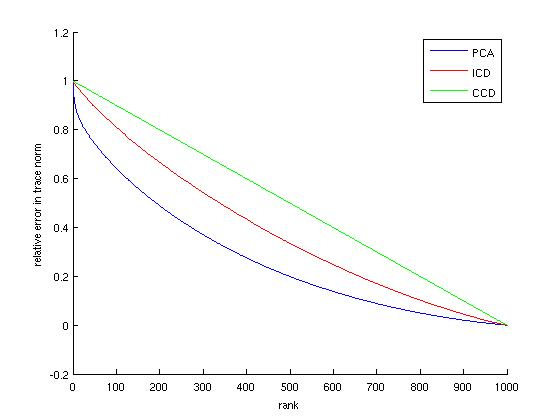
\includegraphics[width=0.5\textwidth]{trace_residual.jpg}
%    \caption{Residual error of decompositions varying by its rank.}
%    \label{fig:residue}
%\end{figure}



\section{Experimental Evaluation}
\label{eval}


\subsection{Datasets and evaluation protocol} \label{eval:protocol}
We perform our experiments in three standard datasets for image retrieval. 
\begin{itemize}
    \item The INRIA \emph{Holidays} dataset \cite{holidays} consists of 1491 images divided in 500 groups of matching images. We manually rotate by 90 degrees some images that are not in their natural orientation to compensate for the fact that CNN features are not rotation invariant~\cite{babenko14,Arandjelovic15,RaToCh16}
    \item The \emph{Oxford5k} dataset \cite{oxford}, which consists of 5063 images separated in 55 groups of matching images, each group associated to a landmark of Oxford. We use the "full" crop, ignoring the region of interest of each image.
    \item The \emph{Oxford105k} dataset \cite{oxford}, large-scale dataset containing the same images and queries from Oxford5k plus \emph{Flickr100k}, a collection of $1e^5$ distractor images Flickr.
\end{itemize}
As pool of negative images to build SLEM, we use the Flickr100k for both Holidays and Oxford5k. When training on Oxford105k, we us instead the \emph{Paris} dataset \cite{PhiChIsSiZi08} as negative samples.
%In both datasets, each group contains one query image, the other images in the group being the only correct answers to the query.
%For each query image, we calculate its similarity to all other images in the database and rank them in decreasing order.
%The average precision of a group is derived from the ranking of the images of the group for the similarity with the corresponding query image.
%The final mean average precision (mAP) for a dataset is the mean of the average precision over all its groups.
%As pool of negative images to build SLEM, we use the Flickr100k collection \cite{oxford}, composed of $10^5$ images from Flickr. For a full rank decomposition, we use only a subset of it, containing between 6000 and 15000 images.
%As stated in section \ref{low-rank} and further discussed in section \ref{time-scale}, a full rank decomposition does not scale well for bigger number of negative samples. For low rank decomposition, we use all 100000 images.

At evaluation time, for a dataset that consists of $p$ images and $q$ query images, we calculate its $p\times q$ \emph{similarity matrix} $S$, where each of its $q$ columns is the matching scores of the query image with all the $p$ images. \hlc{RR: maybe take out this paragraph completely.}


\subsection{Which kernel to choose?}
For the experiment of SLEM as a feature encoder, we tested two different kernels --Gaussian and polynomial-- each with a scalar parameter $\gamma$:
\begin{align}
    k_1(x,y) = e^{-\gamma\|x-y \|^2}; \ 
    k_2(x,y) = x^Ty+\gamma(x^Ty)^2. \label{kernels}
\end{align}
\textbf{Gaussian SLEM.} The radial basis function kernel $k_1$ is a
well known reproducing kernel, used for classification with support vector machines.\\
\textbf{Poly SLEM.} The polynomial kernel $k_2$ is a reproducing kernel often used in natural language processing.
%\textbf{SPM SLEM} The spatial pyramid matching kernel of $L+1$ levels in Equation \ref{k:spm} take as input a set of local descriptors and its location in pyramidal bins \cite{spk}. 


\subsection{Base visual features}
We test our feature encoder for four different base features $x$ in$\mathbb{R}^d$; the hand-crafted VLAD image representation and three learned features derived from the activation coefficients of deep Convolutional Neural Networks.

We use the same VLAD variant of \cite{Delhumeau2013} used in \cite{ZePe15} that relies on densely-extracted rootSIFT \cite{3things} local descriptors, per-cluster, PCA-based rotations, and root normalization. Like \cite{ZePe15}, we use $64$ clusters, for a final feature of size $8192$.

The first CNN-based features we use consist of the activation coefficients of the previous-to-last layer of the AlexNet architecture \cite{Krizhevsky2012}, based on a publicly available pre-trained model \cite{jia2014caffe}. These are also the features used in \cite{ZePe15}.

The Sum-Pooling of Convolutional (SPoC) features \cite{babenko15}, which are tailored specifically for the image retrieval application, consist of spatially-weighted sums of the activations of the last convolutional layer of a 19-layer CNN \cite{SimonZisser15}.

Finally, we use the NetVLAD features \cite{Arandjelovic15}, trained for place recognition. These features are obtained by adding a differentiable version of the VLAD algorithm~\cite{Delhumeau2013} as a layer at the end of a convolutional architecture.


%We revisit the VLAD feature presented in \cite{VLAD} as an example of a hand-crafted representation. First we extract a set $\mathcal{F}$ of local descriptors of the image $I$. We use the 128 dimension RootSIFT \cite{3things} descriptors, extracted densely.
%Then, we hard-assign each descriptor $f$ in $\mathcal{F}$ to the closest among $K$ pre-trained codewords $c_k$, $k\in\{1\cdots K\}$,
%one of $K$ set $\mathcal{C}_k$ of descriptors associated to codewords $\{c_k\}_{1\leq k\leq K}$, 
%and map $f$ to a $\RR^{128K}$ vector
%\begin{equation}
%\phi^{VL}_1(f) = \left[0 \cdots 0\quad \Phi_k^T\frac{(f-c_k)}{\|f-c_k\|} \quad 0 \cdots 0\right],
%\end{equation}
%where $\Phi_k$ is a $128\times 128$ PCA matrix learned on training features mapped to $k$-the codeword.
%associated to descriptors in $\mathcal{C}_k$. 
%The final VLAD representation is the power-normalization and $l_2$ normalization of the sum-pooling of $\phi^{VL}_1$:
%\begin{equation}
%\phi^{VL}_2(I) \propto \mathrm{power}\big(\sum_{f\in \mathcal{F}}\phi^{VL}_1(f)\big),~\|\phi^{VL}_2(I)\|=1,
%\end{equation}
%with scalar power normalization $\mathrm{power}(v)=\mathrm{sign}(v)|v|^{0.2}$ applied component-wise.
%In experiments, we use $K=64$ codewords learned on images from Flickr. Our VLAD representation has $d=8192$ dimensions.

%Convolutional features obtained from very deep convolutional neural networks (CNNs) have been shown to work as good local descriptors for matching \cite{SimonZisser15}. The SPoC representation \cite{babenko15} is a weighted sum-pooling of the activations of the last convolutional layer of a 19-layer CNN. For a given input image $I$, the activations in this layer are organized over a $W\times H$ spatial grid and over $d$ channels. Each position $(w,h)$ in $\{1 \cdots W\}\times \{1\cdots H\}$ can thus be equipped with a descriptor $f_{h,w}(I)$ in $\RR^D$.
%Indeed, if our last convolutional layer has $D$ neurons, and each neuron a $W\times H$ map of activations of this neurons to the image $I$, 
%each pair $(w,h)$ with $w$ in $\{1,2,..., W\}$ and $h$ in $\{1,2,...,H\}$ can be associated to a descriptor $f_{(h,w)}$ in $\RR^D$ of the responses of each neuron at coordinate $(w,h)$ of the maps. 
%We then sum-pool these descriptors, weighted accordingly to their distance to the center of the image:
%\begin{equation}
%    \phi^{SPoC}(I) = \sum_{w=1}^W\sum_{h=1}^H \alpha_{w,h}f_{w,h}(I),
%\end{equation}
%where
%\begin{equation}
%    \alpha_{w,h} = \exp \left(-\dfrac{(w-W/2)^2+(h-H/2)^2}{2\sigma^2}\right).
%\end{equation}
%In our experiments, we follow the implementation details of \cite{babenko15}: We resize all images to $586\times 586$ pixels before feeding them to the network. The last convolutional layer has $d=512$ channels with activation maps of size $(W,H)=(37,37)$, and we set $\sigma=\frac{H}{3}$. We use the same network architecture to extract the convolutional maps but different weights in the convolutional layer, which might explain the difference between the results in Table \ref{fullrank:results} and \cite{babenko15}.

%Finally, we also test a more convencional CNN feature, less deep and using two fully connected layers after the convolutional layers.
%Our final representation is a $4096$ non-negative feature. We based out implementation on CAFFE \cite{jia2014caffe}.



\subsection{Image retrieval results}

We test our method against the original ESVM, PCA and LDA algorithms. The results are presented in Table \ref{fullrank:results}.
\textit{Babenko et al.}~\cite{babenko15} and \textit{Arandjelovi\'c et al.}~\cite{Arandjelovic15} improve the retrieval results applying a PCA compression followed by whitening. 
Thus for these features, we considere their version as presented in \cite{Arandjelovic15,babenko15} in the \textit{PCA+whitening} row and the not-compressed, not-rotated and not-whitened version as \textit{Baseline}. 
For VLAD and AlexNet, we considere the version presented in~\cite{ZePe15} as \textit{Baseline} and a rotated, whitened and compressed to half its original dimensions as \textit{PCA+whitening}. 
As for the version of each feature to which we apply the other algorithms, it changes according to the dataset. 
For SPoC, we apply LDA, ESVM and SLEM to the baseline, as a replacement of PCA. 
For NetVLAD, we use the rotated and compressed version of the trained networks correspondent to each dataset as suggested by~\cite{Arandjelovic15}. 
For Holidays we obtain better results with whitened features and for Oxford5k, non-whitened.

For \textit{LDA}, we follow our description in section \ref{sec:lda} and calculate $\Sigma$ as the convariance of the negative samples.
%In our experiments, the compression worsens the results when compared with non-compressed. \textit{Delhumeau et al.}~\cite{Delhumeau2013}
%Hence we compare the improvements of PCA plus whitening, without compression, with our method.
Linear SLEM performs similarly to ESVM despite being much more time efficient (see discussion in section \ref{time-scale}). 
The fact that a hinge-loss classifier does not outperform a square-loss classifier can seem counter-intuitive, but both were shown to be equivalent for binary classification under mild constraints~\cite{YeXi07}.

We perform both Gaussian SLEM and Polynomial SLEM with two decompositions: one full-rank CCD decomposition signaled by (fr) and two low-rank KPCA decompositions signaled by the rank of the decomposition. 
We train our exemplar classifiers for between $6000$ and $10000$ negative samplers. We outperform all methods, for all datasets and all image representations. \hlc{RR: Do we? I'm putting it here because I'm an optimistic, but we have to wait the results.}


\begin{table*}[h!]
\begin{center}
\setlength{\tabcolsep}{.2em}
%\begin{tabular}{|c|c|c|c|c|c|c|c|}
%\small
\begin{tabular}{c@{\hskip 1em}cccc@{\hskip 1em}cccc@{\hskip 1em}cc}%@{\hskip 1em}c}
\toprule
Dataset & \multicolumn{4}{c}{\textbf{Holidays}} & \multicolumn{4}{c}{\textbf{Oxford 5k}} & \multicolumn{2}{c}{\textbf{Oxford 105k}} \\%& \textbf{Oxford 105k}\\
\midrule
Model, features & VLAD  & SPoC & AlexNet & NetVLAD & VLAD & SPoC & AlexNet & NetVLAD & SPoC & NetVLAD\\% & SPoC\\
\midrule
Baseline            & 72.7 & 76.4 & 68.2  &  85.4 & 46.3 & 54.4 & 40.6 & 67.5 & - & - \\% & 50.1\\
%Whitening           & -    & -    & -    & -    & -\\
PCA+whitening       & 69.4 & 81.6 & 69.2 & 88.3  & 50.9  & 63.7 & 45.0 & 69.1 & - & - \\% & 55.5\\
LDA                 & -   &   -   &  -   &   -   &   -   &   -  & 40.5 &  -  & - & - \\
E-SVM               & 77.5 & 84.0 & 71.3 & 90.5 & 57.2  & 62.1 & 43.9 & 70.4(?) & - & - \\% & 56.5\\ netvlad_hol: 91.6
Linear SLEM         & 78.0   & 82.3 & 72.1 & 90.9& \ul{59.3}  & 64.1 & 46.9/42.2(?) & 72.4 & - & - \\% & 56.7\\
Gaussian SLEM (16)  & - & - & - & 91.1 & - & - & - & 70.8 & - & - \\
Gaussian SLEM (32)  & - & 82.2 & - & 91.0 & - & - & - & 71.1 & - & - \\
Gaussian SLEM (fr)  & 78.1 & 85.2 & \ul{72.9} & 91.4 & 59.0   & \ul{64.9} & 47.0 & \bf{73.2} & - & - \\% & 59.5\\
Poly SLEM (16)      & - & 82.3 & - & 91.3 & - & 63.6 & - & 71.2 & - & - \\
Poly SLEM (32)      & - & 82.4 & - & \bf{91.7} & - & 63.6 & - & 71.7 & - & - \\
Poly SLEM   (fr)    & 78.1 & \ul{86.3}  & \ul{72.9} & \bf{91.7} & \ul{59.3}  & 64.8 & \ul{47.3} & \bf{73.2} & - & - \\% & \bf{62.3}\\
%Zepeda \textit{et al.} \cite{ZePe15} & \underline{78.3} & - & 71.8 & - & 57.5 & - & 44.6 & - & - \\
%Babenko \textit{et al.} \cite{babenko15} & - & 81.8 & - & - & - & \textbf{65.7} & - & - & 57.8\\
\hline
\end{tabular}
\caption{Mean average precision results for INRIA Holidays and Oxford buildings datasets, expressed as percentages. In this table, we present our results for VLAD \cite{Delhumeau2013}, sum-pooling of convolutional features (SPoC) \cite{babenko15}, activation coefficients from the previous-to-last CNN layer (AlexNet) \cite{Krizhevsky2012} and activation of NetVLAD layer~\cite{Arandjelovic15}. In parenthesis, the rank of he decomposition ('fr' for full rank decomposition)}
\end{center}
\label{fullrank:results}
\end{table*}

For all the experiments we calibrate the regularization cost $\lambda$, as well as the parameter $\gamma$. 
%For some experiments, specially using VLAD, the optimal value of $\gamma$ is rather small ($\gamma\sim 0.05$), which suggests the linear kernel is already close to the optimal kernel for these features.



\subsection{Time and storage scalability} \label{time-scale}
In this section we compare the time efficiency of our method and the E-SVM, as well as discuss which method to use accordingly with the number of positive and negative samples.

In Figure \ref{fullrank:results}, we that the see Linear SLEM efficiency does not change with $n$.
Indeed, if $d$ is the dimension of the base representation, $A$ is a $d\times d$ matrix for linear SLEM, whereas for a full rank kernel, $A$ is $n\times n$.
This explains the increasing running time for Gaussian and polynomial kernels: storage and solving a $n\times n$ system does not scale for large number of negative samples.
Retrieval results for kernelized SLEM in Figure \ref{fullrank:results} suggest we can benefit from larger sets of negative samples, but its improvements are not steadily. Indeed, the calculation time for a full rank kernel matrix offline is $O(n^3)$, as it can be seen in Figure \ref{fullrank:results}.
When in consider only the online procedure of our model, \emph{i.e.} the calculation of $\beta^\star$, our kernelized model similarly to ESVM. Therefore, we can process the kernel SLEM for the Gaussian and polynomial kernel similar running time to ESVM if we pre-process our negative samples offline.
For the low-rank decomposition \hlc{not yet presented in Figure \ref{fullrank:results}}, the offline procedure is $O(n^3)$, similarly to the full rank. However this step is much more time consuming for the low-rank, as shown in Figure \ref{fig:residue}. We need test different values of $n$, but for fixed rank $r$, we should expect better results for smaller $n$.    

\vspace{3 mm}

\begin{figure*}
  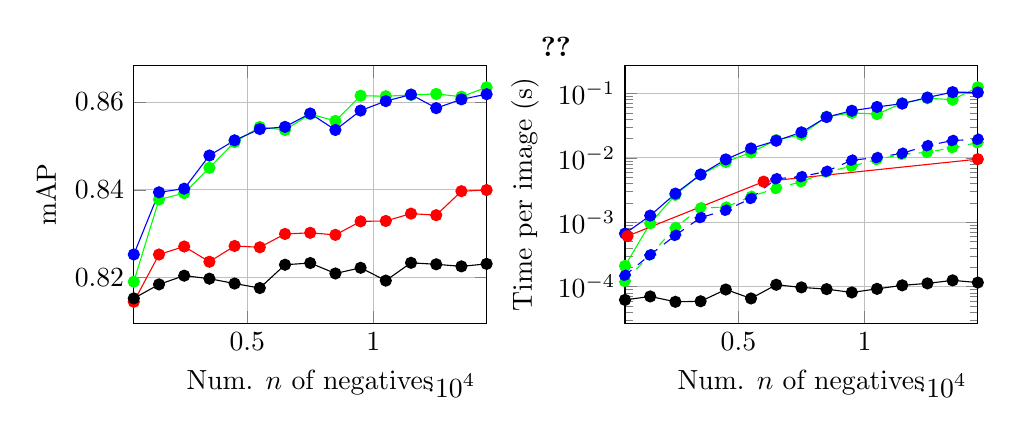
\begin{tikzpicture}
    \begin{groupplot}
      [group style={%
        columns=2,
        rows=1,
        group name=plots,
        xlabels at=edge bottom,
        %y descriptions at=all,
        horizontal sep=5em,        
      },
      % ybar,
      % ymin=0,
      % ymax=27e3,
      enlarge x limits={abs=.5},
      width=0.5\textwidth,
      height=0.4\textwidth,
      % scaled y ticks=base 10:-3,
      % xticklabels from table={\first}{Criterion},
      % x tick label style={rotate=90,anchor=east},
      % xtick=data,
      ]

      \nextgroupplot[xlabel=Num. $n$ of negatives,
      ylabel=mAP]
      ]
      %% Poly SLEM
      \addplot[PolySLEM] coordinates {%gamma=10^-3, lambda=10^-3
        (500,  0.81905)
        (1500, 0.83777)
        (2500, 0.83924)
        (3500, 0.84502)
        (4500, 0.85089)
        (5500, 0.85432)
        (6500, 0.85364)
        (7500, 0.85724)
        (8500, 0.85571)
        (9500, 0.86146)
        (10500,0.86133)
        (11500,0.86163)
        (12500,0.86186)
        (13500,0.86122)
        (14500,0.86336)
      };
      %% Gaussian SLEM
      \addplot[GaussSLEM] coordinates {
        (500,  0.82525)
        (1500, 0.83943)
        (2500, 0.84025)
        (3500, 0.84782)
        (4500, 0.85128)
        (5500, 0.85385)
        (6500, 0.85434)
        (7500, 0.85740)
        (8500, 0.85364)
        (9500, 0.85806)
        (10500,0.86022)
        (11500,0.86172)
        (12500,0.85862)
        (13500,0.86062)
        (14500,0.86180)
      };
      %% ESVM8
      \addplot[ESVM] coordinates {
        (500,  0.81446)
        (1500, 0.82524)
        (2500, 0.82707)
        (3500, 0.82359)
        (4500, 0.82719)
        (5500, 0.82689)
        (6500, 0.82993)
        (7500, 0.83019)
        (8500, 0.82972)
        (9500, 0.83280)
        (10500,0.83289)
        (11500,0.83457)
        (12500,0.83421)
        (13500,0.83968)
        (14500,0.83995)
      };
      %% Linear SLEM
      \addplot[LinSLEM] coordinates {%lambda = 10^-3
        (500,  0.81524)
        (1500, 0.81843)
        (2500, 0.82042)
        (3500, 0.81973)
        (4500, 0.81862)
        (5500, 0.81760)
        (6500, 0.82291)
        (7500, 0.82330)
        (8500, 0.82092)
        (9500, 0.82221)
        (10500,0.81929)
        (11500,0.82335)
        (12500,0.82301)
        (13500,0.82254)
        (14500,0.82311)
      };

      \nextgroupplot[
      ymode=log,
      xlabel=Num. $n$ of negatives,
      ylabel=Time per image (s),
      legend to name=grouplegend,
      legend style={legend columns=-1},
      % legend style={at={(0.465,-0.45)},
      % anchor=north,legend columns=-1},
      ]%
      %% Poly SLEM
      \addplot[PolySLEM] coordinates {
        (500,  0.0002099)
        (1500, 0.0009621)
        (2500, 0.0026628)
        (3500, 0.0054810)
        (4500, 0.0086532)
        (5500, 0.0121226)
        (6500, 0.0188800)
        (7500, 0.0228739)
        (8500, 0.0434941)
        (9500, 0.0499160)
        (10500,0.0477895)
        (11500,0.0703987)
        (12500,0.0842496)
        (13500,0.0802379)
        (14500,0.1245190)
      };
      \addlegendentry{Poly SLEM}
      %% Gaussian SLEM
      \addplot[GaussSLEM] coordinates {
        (500,  0.0006671)
        (1500, 0.0012690)
        (2500, 0.0027834)
        (3500, 0.0055151)
        (4500, 0.0094601)
        (5500, 0.0140014)
        (6500, 0.0184553)
        (7500, 0.0249103)
        (8500, 0.0430012)
        (9500, 0.0539018)
        (10500,0.0617439)
        (11500,0.0695579)
        (12500,0.0865806)
        (13500,0.1049192)
        (14500,0.1037325)
      };
      \addlegendentry{Gaussian SLEM}
      %% ESVM
      \addplot[ESVM] coordinates {
        % (600, .000610)
        % (6000, .00427)
        % (60000, .0378)
         (1000 * 6/10, .000610)%(1000 * 6/10, .002440)
        (10000* 6/10, .00427)%(10000* 6/10, .01708)
        (14500, .0095478)%(14500, .0382) %Interpolated
        % (100000 * 6/10, .0378)
        % (500,  0.014)
        % (1500, 0.015)
        % (2500, 0.016)
        % (3500, 0.017)
        % (4500, 0.018)
        % (5500, 0.019)
        % (6500, 0.02)
        % (7500, 0.021)
        % (8500, 0.022)
        % (9500, 0.023)
        % (10500,0.024)
        % (11500,0.025)
        % (12500,0.026)
        % (13500,0.027)
        % (14500,0.028)
      };
      \addlegendentry{ESVM}
      %% Linear SLEM
      \addplot[LinSLEM] coordinates {
        (500,  0.0000622)
        (1500, 0.0000704)
        (2500, 0.0000581)
        (3500, 0.0000592)
        (4500, 0.0000902)
        (5500, 0.0000655)
        (6500, 0.0001069)
        (7500, 0.0000973)
        (8500, 0.0000914)
        (9500, 0.0000812)
        (10500,0.0000923)
        (11500,0.0001047)
        (12500,0.0001122)
        (13500,0.0001251)
        (14500,0.0001156)
      };
      \addlegendentry{Linear SLEM}
      \addplot[mark=*, green, dashed] coordinates {
            (500,  0.0001208)
            (1500, 0.0003114)
            (2500, 0.0008255)
            (3500, 0.0016757)
            (4500, 0.0017118)
            (5500, 0.0025198)
            (6500, 0.0033489)
            (7500, 0.0042703)
            (8500, 0.0060299)
            (9500, 0.0074267)
            (10500,0.0094138)
            (11500,0.0113405)
            (12500,0.0121783)
            (13500,0.0144320)
            (14500,0.0171987)
          };
      \addplot[mark=*, blue, dashed] coordinates {
            (500,  0.0001501)
            (1500, 0.0003122)
            (2500, 0.0006261)
            (3500, 0.0011822)
            (4500, 0.0015350)
            (5500, 0.0023396)
            (6500, 0.0047356)
            (7500, 0.0051036)
            (8500, 0.0061753)
            (9500, 0.0092072)
            (10500,0.0101006)
            (11500,0.0117932)
            (12500,0.0154758)
            (13500,0.0185985)
            (14500,0.0194114)
          };
      
      


    \end{groupplot}

    \node at (plots c1r1.north east) [anchor=south, xshift=2.5em] {\ref{grouplegend}};
    %\draw (plots c2r1.north west) circle (3pt) node {North west};

  \end{tikzpicture}
  \caption{Results for INRIA Holidays, using SPoC features and different methods of SLEM (see legend). We use $T=10^5$ iterations for all $n$ to report mAP for ESVM, as suggested by \cite{ZePe15}, but report timings using $T=1.66 n$ and the values reported in Table 1 of \cite{ZePe15}. Left: mAP; Right: computation time in solid line, \emph{online} computational cost in dashed line.}
  \label{fullrank:results}
\end{figure*}


\subsection{Comparation to the state of the art}
Results shown in Table~\ref{sota:results}. We do not include re-ranking nor query expansion. 

\begin{table}[t]
\begin{center}
\setlength{\tabcolsep}{.2em}
\small
\begin{tabular}{l|c|ll}
\toprule
Features & dim & \textbf{Hol.} & \textbf{Ox5k} \\%& \textbf{Oxford 105k}\\
\midrule
Babenko \textit{et al.}\cite{babenko15}  & 256 & 80.2 & 58.9 \\ %& 57.8\\
Radenovi\'c \textit{et al.} \cite{RaToCh16}   & 256 & 81.5 & \un{77.4} \\
Arandjelovi\'c \textit{et al.} \cite{Arandjelovic15}& 256 & 86.0 & 62.5 \\ %& - \\
Kalantidis  \textit{et al.} \cite{KaMeOs16}   & 256 & 83.1 & 65.4 \\
SPoC + Linear SLEM & 256 & 82.3 & 64.1 \\
SPoC + Poly SLEM & 288 & 82.3 & 60.6 \\
SPoC + Poly SLEM & 320 & 82.4 & 60.7 \\
NetVLAD + Linear SLEM & 256 & \un{88.5} & - \\
NetVLAD + Poly SLEM & 288 & 87.7 & 65.5 \\
NetVLAD + Poly SLEM & 320 & 88.3 & 65.4 \\
\midrule
Radenovi\'c \textit{et al.} \cite{RaToCh16}   & 512 & 82.5 & 79.7 \\
Arandjelovi\'c \textit{et al.} \cite{Arandjelovic15}& 512 & 86.7 & 65.6 \\
Kalantidis \textit{et al.} \cite{KaMeOs16}   & 512 & 84.9 & 68.2 \\
Gordo \textit{et al.} \cite{GoAlReLa16} & 512 & 89.1^{\dag} & \bf{83.1}^{\dag} \\
NetVLAD + Linear SLEM & 512 & 89.3 & 68.9 \\
NetVLAD + Poly SLEM & 544 & 89.9 & 69.0 \\
NetVLAD + Poly SLEM & 576 & \un{89.9} & 69.2 \\
\midrule
Arandjelovi\'c \textit{et al.} \cite{Arandjelovic15}& 4096 & 88.3 & 69.1 \\
Li \textit{et al.} \cite{LiLaHa15}& - & 89.2^{\dag} & 73.7 \\
NetVLAD + Linear SLEM & 4096 & 90.9 & 72.1 \\
NetVLAD + Poly SLEM & 4128 & 91.3 & 71.2 \\
NetVLAD + Poly SLEM & 4160 & \bf{91.7} & 71.7 \\
%Zepeda \textit{et al.} \cite{ZePe15} & \underline{78.3} & - & 71.8 & - & 57.5 & - & 44.6 & - & - \\
%Babenko \textit{et al.} \cite{babenko15} & - & 81.8 & - & - & - & \textbf{65.7} & - & - & 57.8\\
\hline 
\end{tabular}
\caption{Compared results to state-of-the-art features at similar dimensions, without re-ranking or query augmentation. The results using Poly SLEM or Gaussian SLEMa dd 32 or 64 dimensions to the original feature (for $r=16$ or $r=32$, respectively). Underlined results are the best at each dimension bracket and bold results are the general best. $\dag$ indicates the previous state-of-the-art.}
\end{center}
\label{sota:results}
\end{table}

%\subsection{Semantic correspondence results}

\subsection{Classification results}

%\subsection{Comparison with the state of the art}
\label{sec:sota}
\begin{table}[!t]
  \centering
  \caption{Comparison to state-of-the-art.}
  \label{tbl:sota}
  %\begin{tabular}{|c|c|c|c|c|}
  \setlength{\tabcolsep}{.5em}
  \begin{tabular}{ccccc}
    \toprule
    Dataset & dim &\textbf{Holidays} & \textbf{Oxford 5k} & \textbf{Oxford 105k}\\
    \midrule
    SPoC+GaussianSLEM                           & 1e3  &  81.4           &  \textbf{64.9}  &   -  \\
    SPoC+PCA+PolySLEM                           & 1e3  &  82    &   64.5  &  \textbf{62.3} \\
    Zepeda \textit{et al.} \cite{ZePe15}        & 8e3 &   78.3   &  57.5&  - \\ 
    Babenko \textit{et al.} \cite{babenko15}     & 2e2  &  80.2           &   58.9  &  57.8 \\
    J\'egou \textit{et al.} \cite{sota1}         & -    &  81.3           &    61.5    &   -   \\
    Jain \textit{et al. } \cite{JaJeGro11}       &   -  &  81.9           &    -    &   -   \\
    \midrule
    Tolias \textit{et al.} \cite{Tolias13}      & 1e7  &  \textbf{88}     &  \textbf{82}    &  \textbf{75}   \\
    \bottomrule
  \end{tabular}
  \label{tab:sota}
\end{table}

In Table \ref{tbl:sota} we compare our proposed SLEM architectures to various state-of-the-art methods using a global image representation, as listed in \cite{holidaysSOTA}. 
Note that our method performs comparably to all methods except the very-high dimensional method of Toilas \textit{et al.} \cite{Tolias13} which uses features of size $1e7$.




\section{Conclusion and future work}
\label{conclusion}
In this paper, we address the problem of image retrieval with global image representation. 
We contribute to the domain by presenting a simple idea, the kernelized square loss exemplar machine, and its efficient implementation.
As a result, we obtain significant improvements over the image representations we tested and outperform similar encoders on different datasets. 
As future work, we must work on a convolutional implementation similar to \cite{Arandjelovic15} so its parameters can be learned in a supervised manner.
The use of other kernel functions is worth investigating. The polynomial kernel performs similarly to the Gaussian kernel, even though the Hilbert space obtained from the Gaussian kernel has infinite dimensions and the Hilbert space obtained from the polynomial kernel does not. Different kernels such as the spatial pyramid kernel \cite{spk} are an option for baseline feature that are not global descriptors, wich would increase the versatility of our approach.
%The spatial pyramid kernel can be used to improve representations based on local descriptors and it offers the better boosts when compared with its baseline.




%% RR: uncomment for final version
%% \subsection*{Acknowledgments} This work was supported by the ERC grant VideoWorld.

{\small
\bibliographystyle{ieee} 
\bibliography{sup,jz}
}
\end{document}
